\chapter{Experimentación}
En el capitulo anterior, se presentó de forma general los componentes
más relevantes de la MCE, describiendo entre otros, los mecanismos
para generación de tokens en \(\Lambda\), el mecanismo de traducción
de dichos tokens a acciones en el espacio de acciones \(\mathbb{B}^*\)
y su integración con la capa de cognición de la MCE. 

Sin embargo, aun no se han presentado los agentes que utilizan
esta arquitectura para resolver las tareas propuestas por el usuario.
Formalmente, aun no se ha definido la función \(T_C\bigl(p,\,C^*\bigr) = \lambda\).

Debido a la naturaleza experimental de dicha función, se ha decidido
implementar 8 distintas aproximación agénticas para este problema,
cada una con un enfoque diferente, pero todas compatibles y utilizando
los mecanismos de la MCE.

Nótese que dada la arquitectura propuesta todos los agentes utilizan
el protocolo FastAP para su comunicación con la MCE, lo que los hace
independientes del resto de componentes.

A continuación se describen los agentes implementados, sus
características principales y sus diferencias con el resto de
agentes.

\section{Aproximaciones Agénticas}

A continuación se describen las aproximaciones agénticas
implementadas en la MCE. Es importante denotar que algunos de
estos agentes son variantes de otros, pero con un enfoque
diferente, por lo que se han decidido presentar de forma
separada:

\begin{itemize}
    \item \textbf{Planex}: Basado en el juego de palabras referente 
    a "Planificador Exelent", este es un agente que utiliza un mecanismo de 
    razonamiento y planificación definido en 3 fases. 

    La primera fase genera un plan de acción a largo plazo 
    utilizando acciones perceptivas que le permiten observar 
    el entorno; la segunda fase consiste en una reducción del plan
    generado en un conjunto de acciones que resuelven dicha tarea
    usando acciones dentro del espacio \(\mathbb{B}^*\); la tercera
    fase consiste en la generación de lenguaje exelente para enviarlo
    posteriormente a la capa de Ejecución de la MCE.

    Este agente es integrado dentro de un bucle de control que mantiene
    al agente en un ciclo de observación, planificación y ejecución hasta
    que la tarea sea resuelta o el agente decida detenerse.

    \item \textbf{PlanexV2}: Esta variante de Planex que introduce una fase
    adicional de recuperación. En este sentido, cuando el agente genera halucinaciones
    o errores son recibidos de la capa de ejecución, el agente entra en un bucle
    de recuperación que le permite observar sus propios mensajes, los errores obtenidos
    y reajustar alguna de las 3 fases de Planex para intentar resolver la tarea
    de forma exitosa.

    Este mecanismo permite al agente recuperarse de forma más agil, sin tener que
    realizar una iteración o reinicio completo para poder reaccionar ante errores.

    \item \textbf{RePlan}: Este agente es una variante de Planex que utiliza
    una filosofia de planificación basada en \emph{ReAct}, una de lás metodologías
    de ingeniería de prompting discutida en la sección \ref{sec:prompting}. Así pues,
    ReAct utiliza  un ciclo de razonamiento y acción, donde el agente
    genera un razonamiento sobre la tarea a resolver, seguido de una acción
    que le permite observar y/o modificar su entorno.

    Manteniendo este ciclo de razonamiento y acción, RePlan puede utilizar las capacidades
    de Planex de forma dinámica, decidiendo cuando activar cada fase de Planex de 
    forma autónoma. Con esto, RePlan puede decidir si generar un plan de acción 
    a largo plazo, o generar lenuguaje exelent para enviarlo a la capa de ejecución.


    \item \textbf{Xplore}: Xplore es un agente que utiliza un enfoque de exploración
    y explotación para resolver las tareas propuestas por el usuario. Para ello, Xplore
    utiliza otra técnica de ingeniería de prompting llamada \emph{Grafos Agéntico}. Un
    grafo agéntico consiste en un grafo de acciones y estados, donde cada nodo
    representa un comportamiento del agente, y cada arista representa una transición
    condicional entre comportamientos.

    El grafo agéntico diseñado contempla los estados: planificación a largo plazo,
    planificación a corto plazo, recuperación, aprendizaje y refinamiento. Cada
    uno de estos estados permite representar la información obtenida del entorno en
    distintos formatos, que permitirán a Xplore adaptarse a su entorno y no solo interactuar
    de forma reactiva, sino tambíen modificar su comportamiento a largo plazo a medida
    que su entorno cambia.

    \item \textbf{FastReact}: FastReact es un agente que utiliza un mecanismo
    de razonamiento y acción basado en ReAct, pero con un set de optimizaciones
    que permiten al agente razonar y actuar de formá paralela y mucho más eficiente.

    Este agente ya no utiliza bucles de control, ni esta conectado con Planex,
    sino que directamente es capaz de interactuar con su entorno usando puramente
    lenguaje exelent.

    \item \textbf{Visual-FastReact}: Este agente, abreviado como VFR es una variante
    de FastReact que integra capacidades de visión para obtener no solo información
    desde el espacio de acciones, sino también desde imagenes o capturas de pantalla 
    del entorno.

    De esta forma, VFR puede observar su entorno de forma más completa,
    obteniendo información visual que resulta imposible de obtener
    únicamente con el espacio de acciones \(\mathbb{B}^*\).

    \item \textbf{MinimalVFR}: MinimalVFR es una variante de Visual-FastReact
    que simplifica su arquitectura manteniendo el núcleo del ciclo de
    razonamiento y acción.
    
    A nivel técnico, el agente prescinde de herramientas de flujo como LangGraph
    y basa su ejecución en una arquitectura modular, con métodos claramente
    separados y reemplazables que pueden ser sobreescritos para extender su comportamiento.

    Esta unificación del ciclo cognitivo permite reducir la complejidad y
    aumentar la flexibilidad del agente, facilitando el desarrollo de nuevas
    variantes y mejorando la adaptabilidad a distintos entornos.
    
    \item \textbf{DarkVFR}: DarkVFR es una variante de MinimalVFR que optimiza
    el proceso de extracción de información visual, eliminando información
    irrelevante y enfocándose únicamente en la información que esta relacionada
    con la tarea a resolver.

    A su vez, DarkVFR integra meta-acciones para controlar su comportamiento, así
    como un set de optimizaciones a nivel de memoria que le permiten eliminar
    información textual que puede no ser conveniente para la tarea a resolver.

\end{itemize}

Estos agentes han sido implementados utilizando los mecanismos de ingeniería de prompting
presentados en la sección \ref{sec:prompting}, así como mecanismos de control de mensajes,
llamada a funciones o estructuración de prompts presentados en la sección \ref{sec:canonical_mechanisms}.

Para el desarrollo de los agentes, se ha utilizado la librería \texttt{Langchain} y \texttt{Langgraph}, 
asi como modulos customizados para cada agente escritos totalmente en Python.

\section{Características Técnicas y Funcionales}
A continuación, se presentan las características técnicas y funcionales de cada
agente, seguidas de un análisis comparativo que permitirá formular hipótesis
sobre su comportamiento esperado en distintos escenarios.


\begin{table}[!h]
\centering
\caption{Tipo de Ciclo Cognitivo}
\begin{tabular}{p{3.5cm} p{10cm}}
\toprule
\textbf{Agente} & \textbf{Ciclo Cognitivo Principal} \\
\midrule
\textbf{Planex} & Observación, planificación y ejecución \\
\textbf{PlanexV2} & Observación, planificación, ejecución + recuperación \\
\textbf{RePlan} & ReAct + Planex \\
\textbf{Xplore} & Grafo de comportamientos \\
\textbf{FastReact} & ReAct optimizado \\
\textbf{VFR} & ReAct optimizado + capacidades visuales \\
\textbf{MinimalVFR} & React optimizado + capacidades visuales \\
\textbf{DarkVFR} & React optimizado + capacidades visuales eficientes \\
\bottomrule
\end{tabular}
\end{table}


Esta tabla presenta la clasificación de los agentes en función del tipo de ciclo
cognitivo que estructura su comportamiento. Esta característica define la forma
en que el agente percibe, planifica y actúa sobre el entorno.

Se identifican tres corrientes principales:

\begin{itemize}
  \item \textbf{Ciclo predeterminado (Planex, PlanexV2)}: Estos
  agentes siguen un flujo fijo de observación, planificación y ejecución. Aunque
  este enfoque facilita el control y la predicción del comportamiento, también lo
  hace vulnerable a errores no previstos en fases tempranas.

  \item \textbf{Grafo de comportamientos (Xplore)}: Representa una estructura más
  dinámica, en la que el agente transiciona entre diferentes comportamientos según
  condiciones del entorno. Esto le permite adaptarse mejor a cambios y aprender
  patrones de interacción, aunque requiere un diseño que contemple de forma efectiva
  los estados más representativos de la tarea a resolver.

  \item \textbf{Razonamiento tipo ReAct (RePlan, FastReact, etc.)}: Estos agentes generan decisiones a través de ciclos de
  razonamiento y acción. Son altamente adaptativos y no requieren un flujo
  predefinido, aunque pueden ser menos predecibles y más sensibles a errores de
  generación.
\end{itemize}

\begin{table}[!h]
\centering
\caption{Modularidad y Capacidades Internas de los Agentes}
\begin{tabular}{
  p{2cm}
  >{\centering\arraybackslash}p{2cm}
  >{\centering\arraybackslash}p{0.8cm}
  >{\centering\arraybackslash}p{2cm}
  >{\centering\arraybackslash}p{1.2cm}
  >{\centering\arraybackslash}p{1.6cm}
  >{\centering\arraybackslash}p{1.5cm}
}
\toprule
{\small\textbf{Agente}} & {\small\textbf{Modularidad}} & {\small\textbf{Visión}} & {\small\textbf{Recuperación}} & {\small\textbf{Memoria}} & {\small\textbf{Aprendizaje}} & {\small\textbf{Meta-acciones}} \\
\midrule
\textbf{Planex} & Media & -- & -- & -- & -- & -- \\
\textbf{PlanexV2} & Media & -- & \checkmark & -- & -- & -- \\
\textbf{RePlan} & Alta & -- & \checkmark & \checkmark & -- & -- \\
\textbf{Xplore} & Media & \checkmark & \checkmark & \checkmark & \checkmark & -- \\
\textbf{FastReact} & Alta & -- & \checkmark & \checkmark & -- & -- \\
\textbf{VFR} & Alta & \checkmark & \checkmark & \checkmark & -- & -- \\
\textbf{MinimalVFR} & Muy alta & \checkmark & \checkmark & \checkmark & -- & -- \\
\textbf{DarkVFR} & Muy alta & \checkmark & \checkmark & \checkmark & -- & \checkmark \\
\bottomrule
\end{tabular}
\end{table}

Esta nueva tabla complementa la anterior describiendo aspectos internos clave que
determinan el grado de autonomía, adaptabilidad y extensibilidad de cada agente.
Estas características permiten entender no solo cómo están construidos, sino qué
tipo de comportamiento podríamos esperar cuando se enfrentan a tareas reales.

\begin{itemize}
    \item \textbf{Modularidad}: La evolución de los agentes refleja
    un diseño cada vez más flexible. Mientras Planex y Xplore conservan una
    modularidad media, agentes como MinimalVFR y DarkVFR alcanzan una arquitectura
    altamente desacoplada, facilitando su extensión y mantenimiento.

    \item \textbf{Visión}: Solo Xplore y los agentes de la familia VFR incorporan
    percepción visual, lo que les otorga una ventaja clara en tareas que requieren
    interpretar información del entorno más allá del canal textual.

    \item \textbf{Recuperación}: Excepto Planex, todos los agentes incorporan algún
    tipo de mecanismo para recuperarse de errores. Esto sugiere que, en escenarios
    no deterministas o propensos a fallos, la mayoría de agentes tendrá al menos una
    vía de corrección.

    \item \textbf{Memoria}: Se observa un aumento progresivo en la capacidad de
    memoria. Los agentes más avanzados no solo conservan información entre pasos,
    sino que la reutilizan y modifican activamente para razonar o tomar decisiones futuras.

    \item \textbf{Aprendizaje}: Xplore destaca por incorporar mecanismos
    de aprendizaje. Esto lo posiciona como un candidato adecuado para tareas
    iterativas o con entornos parcialmente observables, donde la adaptación continua
    es una ventaja competitiva.

    \item \textbf{Meta-acciones}: Únicamente DarkVFR tiene la
    capacidad de autorregular su comportamiento mediante meta-acciones.
    Al igual que con Xplore, esto le supone una ventaja competitiva en
    tareas donde la adaptabilidad y la auto-optimización son
    cruciales.
\end{itemize}

En conjunto, la tabla muestra una evolución clara desde agentes básicos y
estructurados hacia otros más modulares, perceptivos y adaptativos. Esta
progresión plantea una pregunta central que será abordada en los siguientes
experimentos:

\emph{¿Realmente estas capacidades avanzadas se traducen en un mejor
rendimiento en tareas prácticas?}

\section{Hipótesis del Experimento}
En las posteriores secciones, se presentarán los entornos de pruebas
diseñados para evaluar el rendimiento de los agentes, así como las métricas
de rendimiento que se utilizarán para medir su eficacia. 

La hipótesis central que se plantea con estos experimentos es que los agentes
desarrollados no solo son capaces de operar de forma autónoma, sino que además
logran integrarse correctamente con la MCE siguiendo la función de cognición 
definida en el modelo teórico. En este sentido, se espera que la interacción 
entre los agentes dentro de la MCE sea equivalente a la función
\(T_C\bigl(p,\,C^*\bigr) = \lambda\), donde \(p\) es el problema a resolver que se
planteara en el entorno de pruebas, \(C^*\) es equivalente al agente
y \(\lambda\) es el lenguaje excelente generado por los agentes para resolver dicho
problema. 


Con esto, el objetivo del experimento no se limita a medir el rendimiento 
individual de cada agente, sino también a evaluar la validez del modelo 
teórico global, entendido como la interacción coordinada de cada uno de los componentes 
dentro de un sistema cognitivo funcional. Las métricas de rendimiento 
obtenidas en estos entornos permitirán valorar tanto la eficacia de cada agente 
como la viabilidad práctica de la MCE como arquitectura agéntica integrada.

\section{Entorno de Pruebas y Evaluación}
Para evaluar el rendimiento de los agentes, se han diseñado 3 entornos
de pruebas que integrarán a cada agente dentro de la MCE. A su vez, este
será desplegado de forma local en un ordenador convencional con un sistema
operativo Windows 11, sin acceso a la GPU, con acceso a internet y
con configuraciones y programas aleatorios, para simular un entorno realista y 
no controlado.

Los objetivos planteados en cada uno de estos entornos son los siguientes:

\begin{enumerate}


  \item \textbf{Hello World}: Este entorno de pruebas cuenta
  con un editor de texto abierto y preparado para recibir entradas de texto.
  El objetivo del agente es escribir el texto \texttt{"Hola Mundo"} en dicho editor,
  Con esta tarea se pretende evaluar la capacidad del agente para interactuar
  con su entorno utilizando el espacio de acciones. 
  
  La métrica de rendimiento más relevante será en este caso será el tiempo que tarda el agente
  en completar la tarea, tratándose esta de una tarea sencilla que puede
  ser directamente resuelta con una única acción.

  Para realizar esta tarea, el agente deberá ser capaz de realizar todas
  las acciones necesarias, habiendo recibido como entrada el siguiente texto:
  \begin{quote}
    \texttt{"Por favor, escribe 'Hola Mundo'"}
  \end{quote}

  \item \textbf{Play a Song}: En este entorno, el agente tendra Spotify
  abierto y preparado con una canción aleatoria. Sin embargo, esta aplicación
  se encontrará minimizada, por lo que el agente deberá encontrar la
  aplicación, maximizarla y reproducir la canción. 
  
  Es importante denotar que esta tarea no requiere de forma obligatoria 
  de capacidades de visión, ni de control de mouse, pues el agente puede descubrir que presionando la 
  tecla \texttt{Espacio} se reproduce la canción, y que la aplicación
  es accesible desde la barra de tareas de Windows.

  Con esta tarea se pretende evaluar la capacidad del agente no solo para 
  interactuar con su entorno, sino también para analizar el estado del mismo 
  y descubrir acciones que le permitan resolver la tarea de forma efectiva.
  En este caso, la métrica de rendimiento no solo será el tiempo que tarda
  el agente en completar la tarea, sino también el número de acciones
  que ha realizado para resolverla, así como si ha sido capaz de resolver
  la tarea. No se evaluará si se han utilizado o no capacidades de visión. 

  La entrada que recibirá el agente para esta prueba será:
  \begin{quote}
    \texttt{"Reproduce una canción en Spotify"}
  \end{quote}

  \item \textbf{Buy on Amazon}: En este entorno el agente iniciará
  en el escritorio de Windows. Tendra aplicaciones abiertas como
  Spotify o Visual Studio Code, pero no tendra ningún navegador abierto.
  El objetivo del agente será: descubrir que navegador tiene instalado,
  abrirlo, encontrar una pagina web de Amazon que tenga un producto
  especificado y o bien añadirlo al carrito de la compra, o bien
  comprarlo directamente con el botón de "Compra en un click"

  Las métricas de rendimiento mas relevantes en este caso serán 
  la eficiencia del agente para realizar la tarea, donde dicha eficiencia
  se medira tanto en el número de acciones como en la cantidad de tokens
  utilizados (en el proceso de razonamiento dentro de la LLM) para completar
  la tarea. 

  Esta tarea es mucho más compleja que las anteriores, pues
  requiere de capacidades de razonamiento, planificación y descubrimiento
  de acciones de forma continuada, dinámica y efectiva.
  A su vez, el agente deberá ser capaz de interactuar con el navegador
  y con la página web de Amazon, lo que implica que deberá ser capaz
  de interpretar el contenido de la página, identificar los elementos
  relevantes y realizar acciones sobre ellos, como hacer clic en botones
  o rellenar formularios.

  La entrada que recibirá el agente para esta prueba será:
  \begin{quote}
    \texttt{"Busca un portatil en Amazon y compralo o añadelo al carrito."}
  \end{quote}

\end{enumerate}

Notese que como medida de seguridad, los agentes contarán con un limite
de tiempo y acciones para completar cada una de estas tareas. Estas
restricciones están diseñadas para evitar que los agentes se queden
atrapados en bucles infinitos o realicen acciones no deseadas.

El tiempo máximo para completar las tareas será de 2.5 minutos para la prueba
de \emph{Hello World}, 5 minutos para la prueba de \emph{Play a Song} y
10 minutos para la prueba de \emph{Buy on Amazon}.

La cantidad máxima de acciones que podrá realizar el agente
será de 3 acciones para la prueba de \emph{Hello World}, 10 acciones
para la prueba de \emph{Play a Song} y 50 acciones para la prueba de
\emph{Buy on Amazon}.

Debido a la naturaleza de cada agente, las acciones que requieran de 
capacidades de visión y/o meta-acciones solo estarán disponibles para aquellos
agentes que sean compatibles con ellas, mientras que el resto de agentes no tendrán
dichas acciones dentro de su espacio de acciones \(\mathbb{B}^*\).

\section{Resultados de la Evaluación}
En esta sección se presentan las métricas, resultados y observaciones obtenidas
durante la evaluación de los agentes en los entornos de pruebas diseñados.

Con este fin, a continuación se analizará por separado el rendimiento general
de cada uno de los entornos junta al impacto de capacidades como visión o recuperación
en el rendimiento de los agentes para finalmente, presentar una comparativa global
de cada uno de los agentes y las conclusiones obtenidas de los experimentos.

\subsection{Rendimiento por Entorno de Pruebas}
Los tres entornos de pruebas han sido diseñados cada uno con una complejidad
incremental, permitiendo evaluar no solo la capacidad de los agentes para
interactuar con su entorno, sino también su habilidad para razonar, planificar
y adaptarse a situaciones cambiantes.

A continuación se presentan los resultados obtenidos en cada uno de los entornos
de pruebas:

\subsubsection{Hello World}
El entorno más sencillo es el de \emph{Hello World}, donde los agentes
deben escribir un texto específico en un editor. 
El prompt de entrada para este entorno es el siguiente:

\begin{quote}
    \texttt{"Por favor, escribe 'Hola Mundo'."}
\end{quote}

Es importante resaltar como dado el prompt de entrada, no se especifica si 
previamente hay un editor abierto, ni si la escritura se puede realizar
directamente de forma satisfactoria. Así pues, dado el prompt, la evaluación
realizada distingue dos comportamientos diferentes:

\begin{itemize}
    \item \textbf{Escritura directa}: El agente escribe el texto directamente
    en el editor, sin comprobar si esta va a ser satisfactoria. Tras esto, 
    puesto que se asume que el editor está abierto, se considera que la tarea
    ha sido completada de forma satisfactoria.

    Aunque este comportamiento es el más eficiente, no puede considerarse
    óptimo, pues se asume información que no se ha proporcionado en el prompt,
    lo que puede llevar a errores si el entorno no es el esperado.

    Este es el caso, por ejemplo, de \emph{Planex}, que en ninguna de las
    pruebas realizadas ha ejecutado acciones adicionales, pero ha completado
    la tarea satisfactoriamente con un tiempo promedio de \emph{13.15s},
    utilizando \emph{1 acción}.

    También agentes como \emph{PlanexV2} y \emph{RePlan} completan la
    tarea con escritura directa, aunque con una ligera variabilidad en tiempo
    (PlanexV2: \emph{13.39s}; RePlan: entre \emph{6.52s} y \emph{15.33s})
    y tokens utilizados.


    \item \textbf{Acciones previas}: El agente realiza acciones adicionales
    para abrir un editor o revisar si en pantalla se encuentra algun programa
    de texto abierto. Tras esto, escribe el texto solicitado
    en el editor. Este comportamiento es más robusto, pues no asume
    información que no se ha proporcionado en el prompt, pero requiere de un
    balance entre eficiencia y robustez, ya que puede requerir más acciones
    para completar la tarea.

    En algunos casos, como con \emph{Xplore}, el agente utiliza acciones de revisión
    de programas abiertos para la verificación, pero sufre de un sobre-esfuerzo:
    en una ejecución llegó a usar \emph{5 acciones} alcanzando los \emph{24.17s} 
    de ejecución, aunque en otras pruebas fue más eficiente reduciendo hasta \emph{2 acciones}
    en \emph{8.97s}.

    Por el contrario, los agentes basados en \emph{FastReact} (incluyendo VFR y DarkVFR)
    demuestran una ejecución eficiente y robusta. Por ejemplo, \emph{DarkVFR}
    logra tiempos por debajo de \emph{5.1s} en promedio, usando únicamente 
    \emph{2 acciones}. Estos agentes alcanzan así un balance adecuado entre 
    robustez y eficiencia, integrando fases de verificación sin sacrificar 
    velocidad de ejecución ni simplicidad del plan de acción.
  
\end{itemize}

La siguiente gráfica muestra el rendimiento de cada agente en el entorno
de \emph{Hello World}:

\begin{figure}[!h]
    \centering
    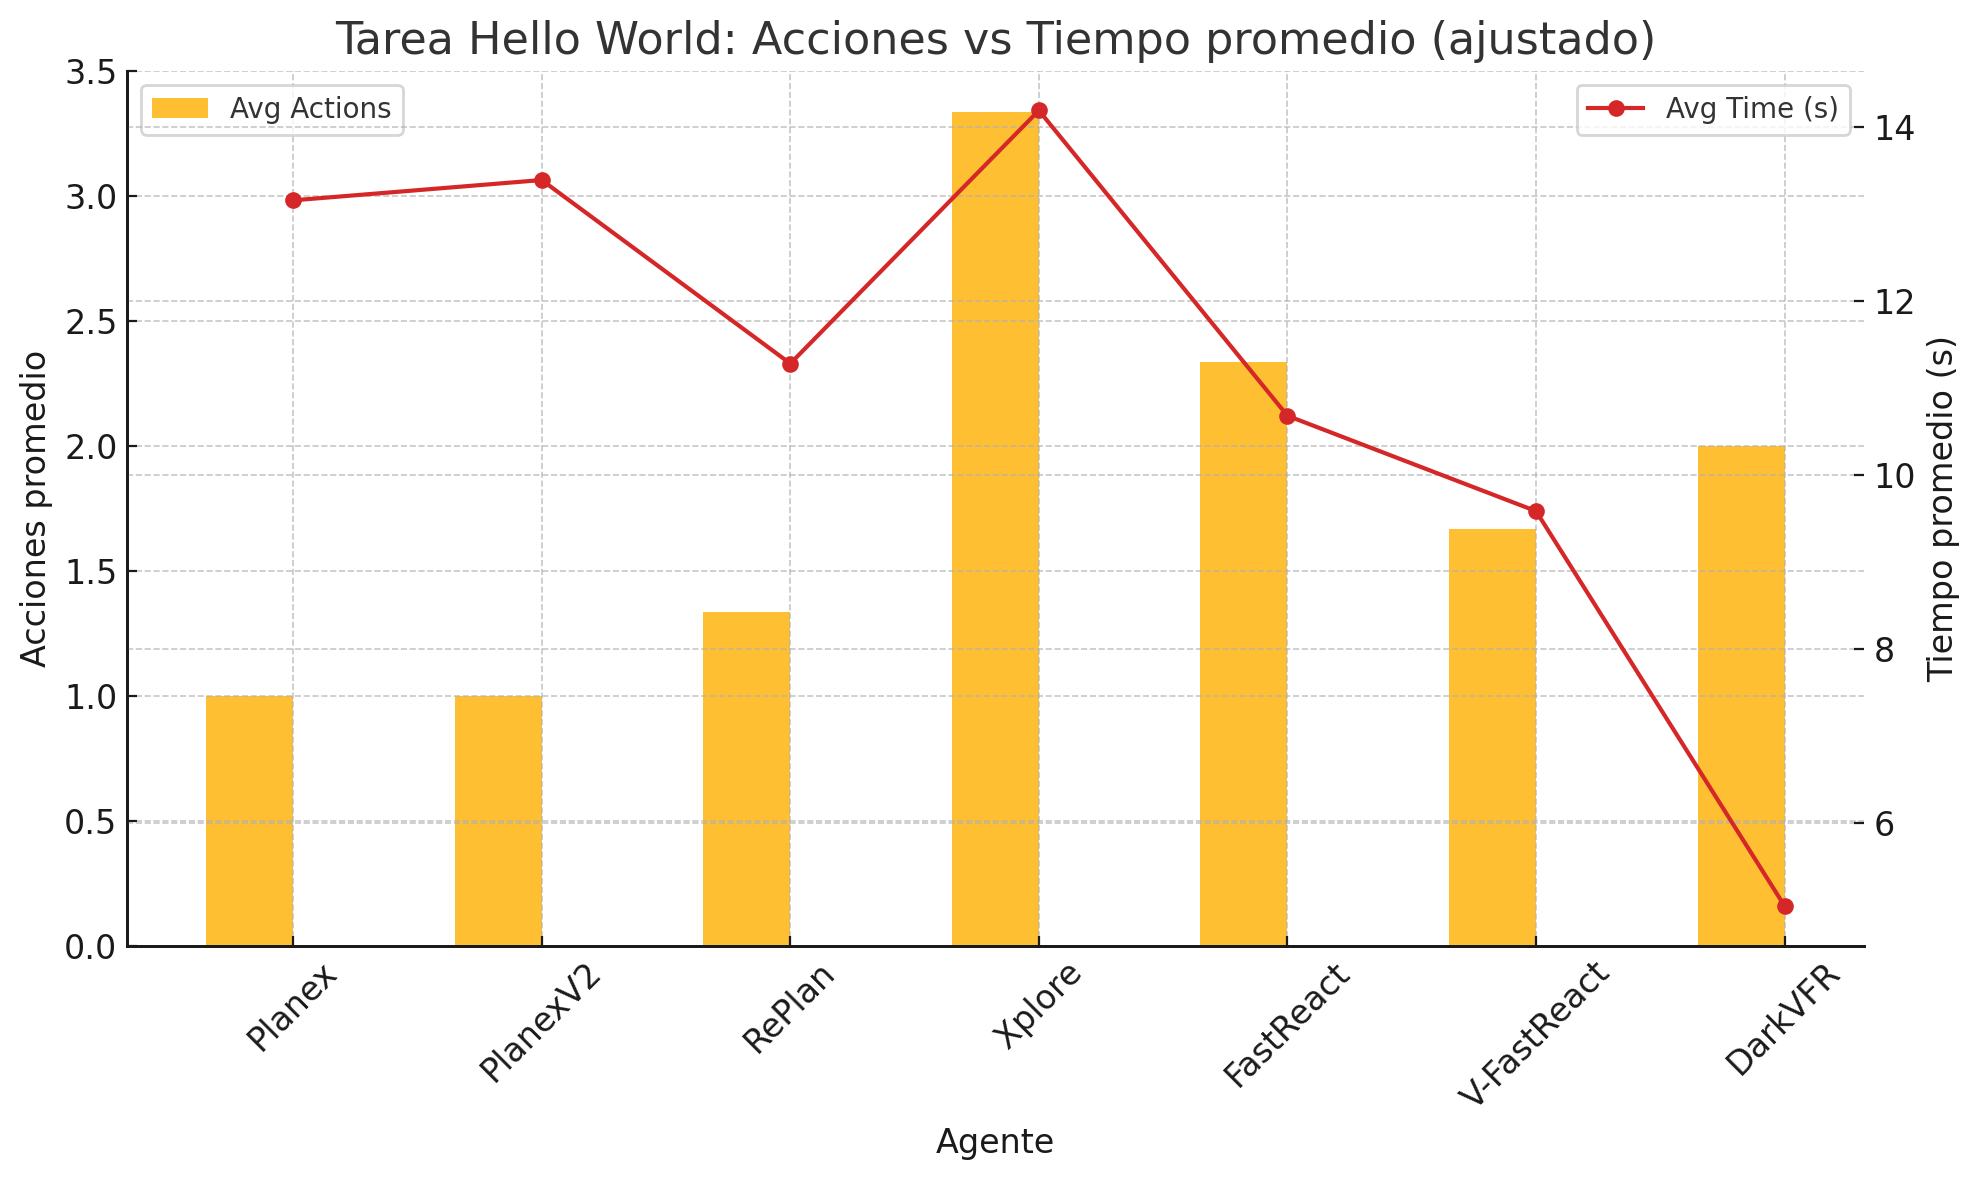
\includegraphics[scale=0.55]{figs/metrics-env-1.png}
    \caption{\small Rendimiento de los agentes (N. Acciones vs Tiempo promedio) en el 
    entorno \emph{Hello World}. Fuente: Elaboración propia.}
    \label{fig:env-1}
\end{figure}

En la figura \ref{fig:env-1} se puede observar como los agentes
mas simples (\emph{Planex}, \emph{PlanexV2} y \emph{RePlan}) logran completar la tarea
con un númmero reducido de acciones, utilizando una estrategia más
directa y asumiendo que el editor ya está abierto. 

También observamos como los agentes basados en React o Fast-React
son más eficientes temporalmente, ahorrando tiempo y recursos gastados
en planificación en contraste con el caso de \emph{Xplore} que alcanza
los \emph{14 segundos} en promedio.

Finalmente también se observa FastReact tienen un rendimiento que balancea
la eficiencia y robustez, logrando completar la tarea en un tiempo
menor al resto de agentes y con un número de acciones reducido.

\begin{figure}[!h]
    \centering
    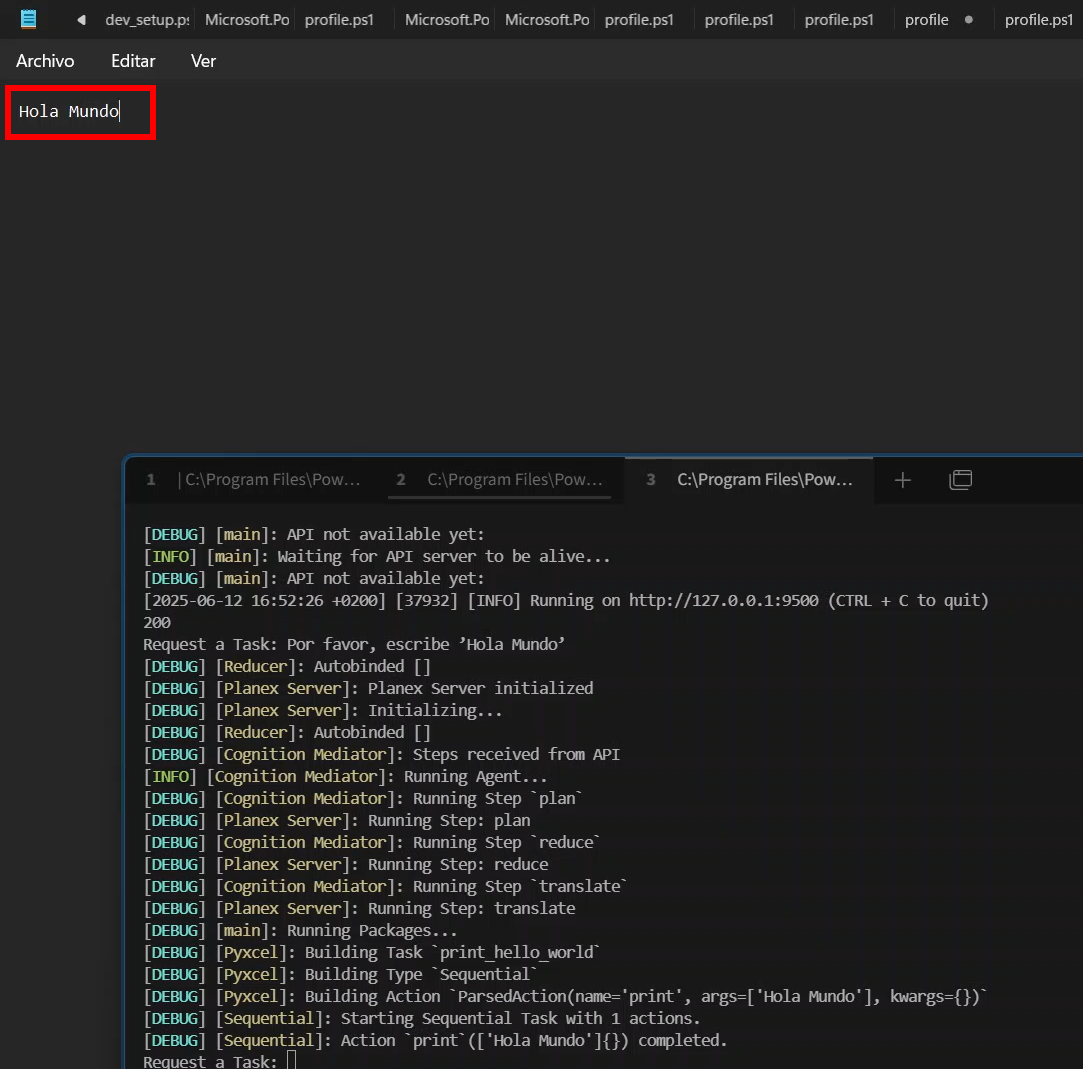
\includegraphics[scale=0.45]{figs/result-env-1.png}
    \caption{Resultado de la evaluación \emph{Hello World} usando Planex. Texto escrito resaltado en un recuadro rojo. Fuente: Elaboración propia.}
    \label{fig:env-1-result}
\end{figure}

\subsubsection{Play a Song}
El entorno de \emph{Play a Song} es más complejo, ya que requiere
que el agente interactúe con una aplicación minimizada (Spotify) y descubra
cómo reproducir una canción. El prompt de entrada para este entorno es:

\begin{quote}
    \texttt{"Reproduce una canción en Spotify."}
\end{quote}

En este caso los siguientes comportamientos se han observado:

\begin{itemize}
    \item \textbf{Abrir Spotify}: En el caso de \emph{Planex} y \emph{PlanexV2}
    los agentes intentan reproducir la canción sin abrir Spotify, siguiendo
    de forma literal el prompt de entrada. Esto provoca que la tarea
    no se complete, ya que no se ha abierto la aplicación. 

    Por el contrario, el resto de agentes, son capaces de recuperarse y descubrir
    que Spotify no está abierto. De forma aleatoria, algunos agentes han decidido
    abrir Spotify directamente, mientras que en otras ejecuciónes han encontrado
    la aplicación en la barra de tareas y la han maximizado.

    \item \textbf{Reproducción de la canción}: Una vez Spotify está abierto,
    existen dos formas de reproducir la canción, o bien haciendo clic en el 
    botón de reproducción, o bien presionando la tecla \texttt{Espacio} en 
    el teclado.

    En el caso de los agentes que no poseen capacidades de visión, como
    \emph{RePlan} se ha observado que en algunos de los intentos, el agente
    descubre que puede presionar la tecla \texttt{Espacio} y completa la tarea,
    sin embargo este obstaculo resulta un bloqueo que ha impedido el completado
    de la tarea en la mayoría de sus casos.

    Por el contrario, los agentes que poseen capacidades de visión, como
    \emph{VFR} o \emph{Xplore} han conseguido completar la tarea de forma
    satisfactoria, ya que han podido observar el botón de reproducción
    y hacer clic en él, o bien presionar la tecla \texttt{Espacio} al revisar
    que la canción se encuentra abierta.

\end{itemize}

\begin{figure}[!h]
    \centering
    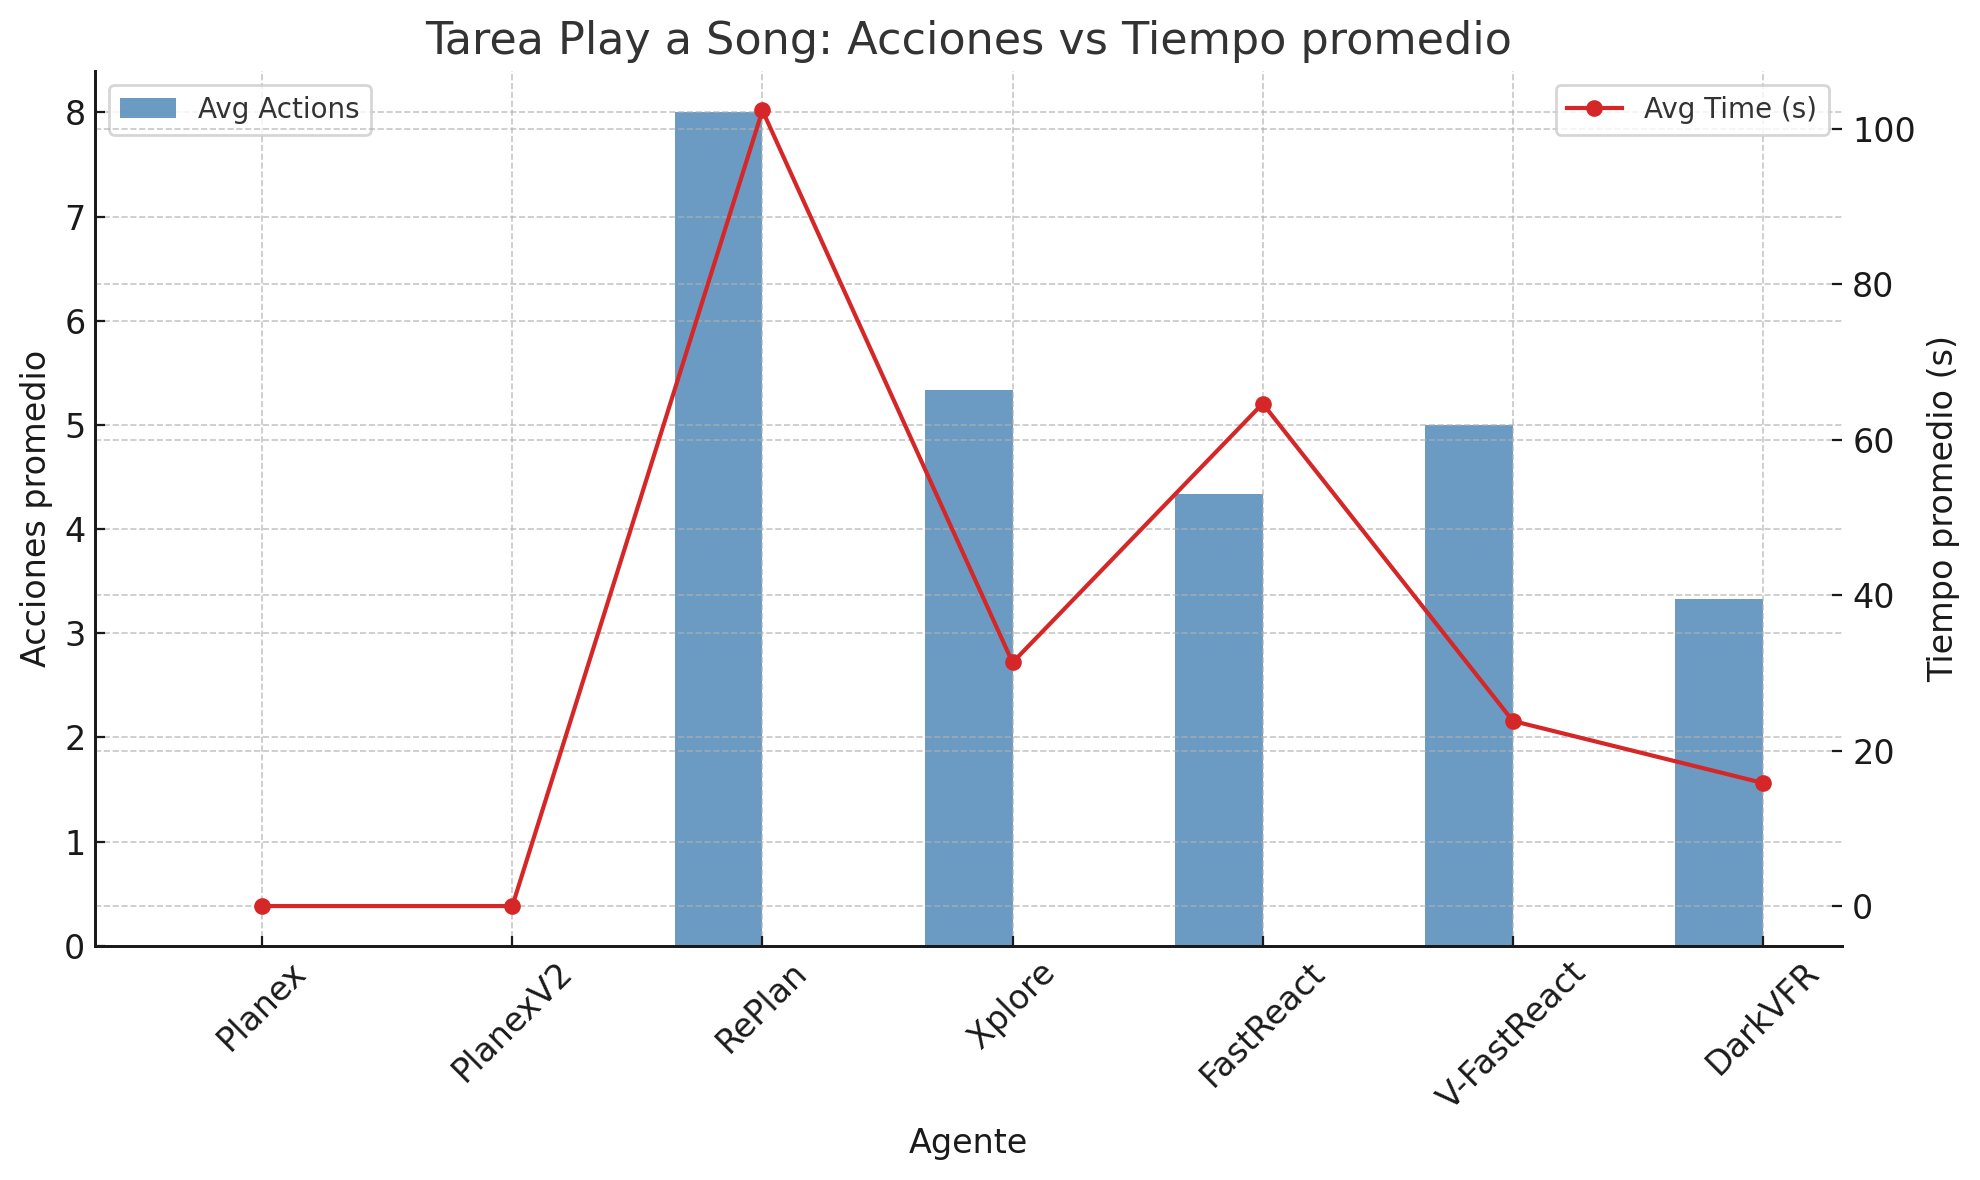
\includegraphics[scale=0.16]{figs/metrics-env-2.png}
    \caption{\small Rendimiento de los agentes (N. Acciones vs Tiempo promedio) en el 
    entorno \emph{Play a Song}. Fuente: Elaboración propia.}
    \label{fig:env2}
\end{figure}

En la figura \ref{fig:env2} se puede observar como los agentes
que no poseen capacidades de visión como \emph{FastReact} o \emph{RePlan} tienen un 
rendimiento inferior al resto de agentes, requiriendo de un mayor tiempo de computo
a analizar posibles métodos de recuperación.

Adicionalmente, \emph{PlanexV2} la capacidad de recuperación no es suficiente
para completar la tarea, al no disponer de una memoria que le permita analizar
con profundidad el estado del entorno y descubrir acciones que le permitan
resolver la tarea de forma satisfactoria.

En el caso del resto de agentes, se observa como completan la tarea 
satisfactoriamente en un tiempo inferior a los \emph{40 segundos} y \emph{6 acciones}.

\begin{figure}[!h]
    \centering
    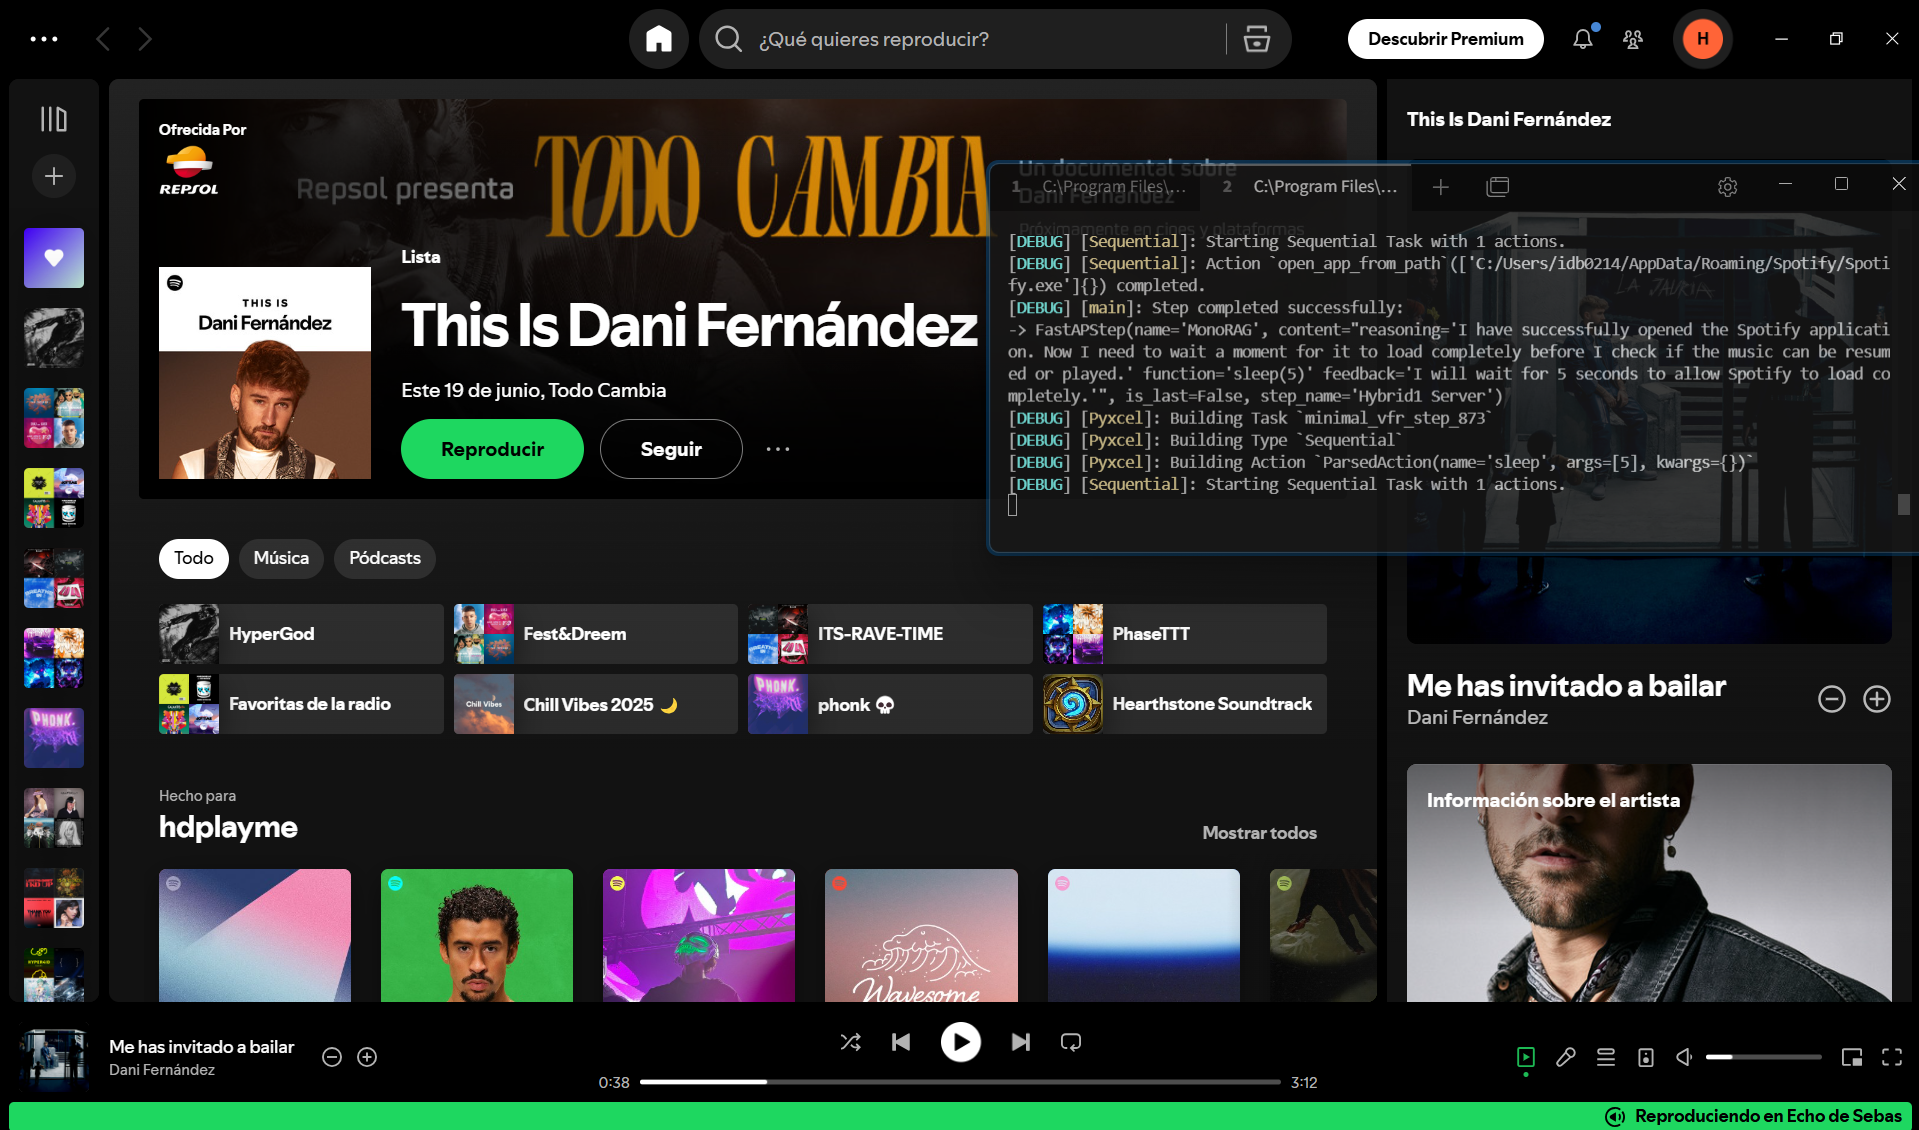
\includegraphics[scale=0.25]{figs/result-env-2.png}
    \caption{VisualFastReact maximizando Spotify para reproducir la canción. Fuente: Elaboración propia.}
    \label{fig:env-2-result}
\end{figure}

\subsubsection{Buy on Amazon}
El entorno de \emph{Buy on Amazon} es el más complejo, ya que requiere
que el agente descubra un navegador, abra una página de Amazon, busque un
producto específico y lo añada al carrito o lo compre directamente. El prompt de entrada
para este entorno es:

\begin{quote}
    \texttt{"Busca un portatil en Amazon y compralo o añadelo al carrito."}
\end{quote}

Nótese que en este caso, no se avisa al agente de que el navegador no se
encuentra abierto. A su vez,
 tampoco se especifica que navegadores se deben
utilizar ni en que sistema operativo se esta trabajando ( en windows, por
ejemplo, se puede utilizar Microsoft Edge, mientras que en Linux se puede
utilizar Firefox o Chrome).

Adicionalmente como se muestra en la figura \ref{fig:laptops}, en busquedas realizadas por los agentes, 
se ha observado como incluso habiendo estos utilizado la búsqueda \emph{laptops site:amazon.com}, los resultados
de la búsqueda no contienen unicamente productos de Amazon, sino que son mayoritariamente anuncios de 
otras páginas, que el agente deberá ignorar o recuperarse para completar la tarea.


\begin{figure}[!h]
    \centering
    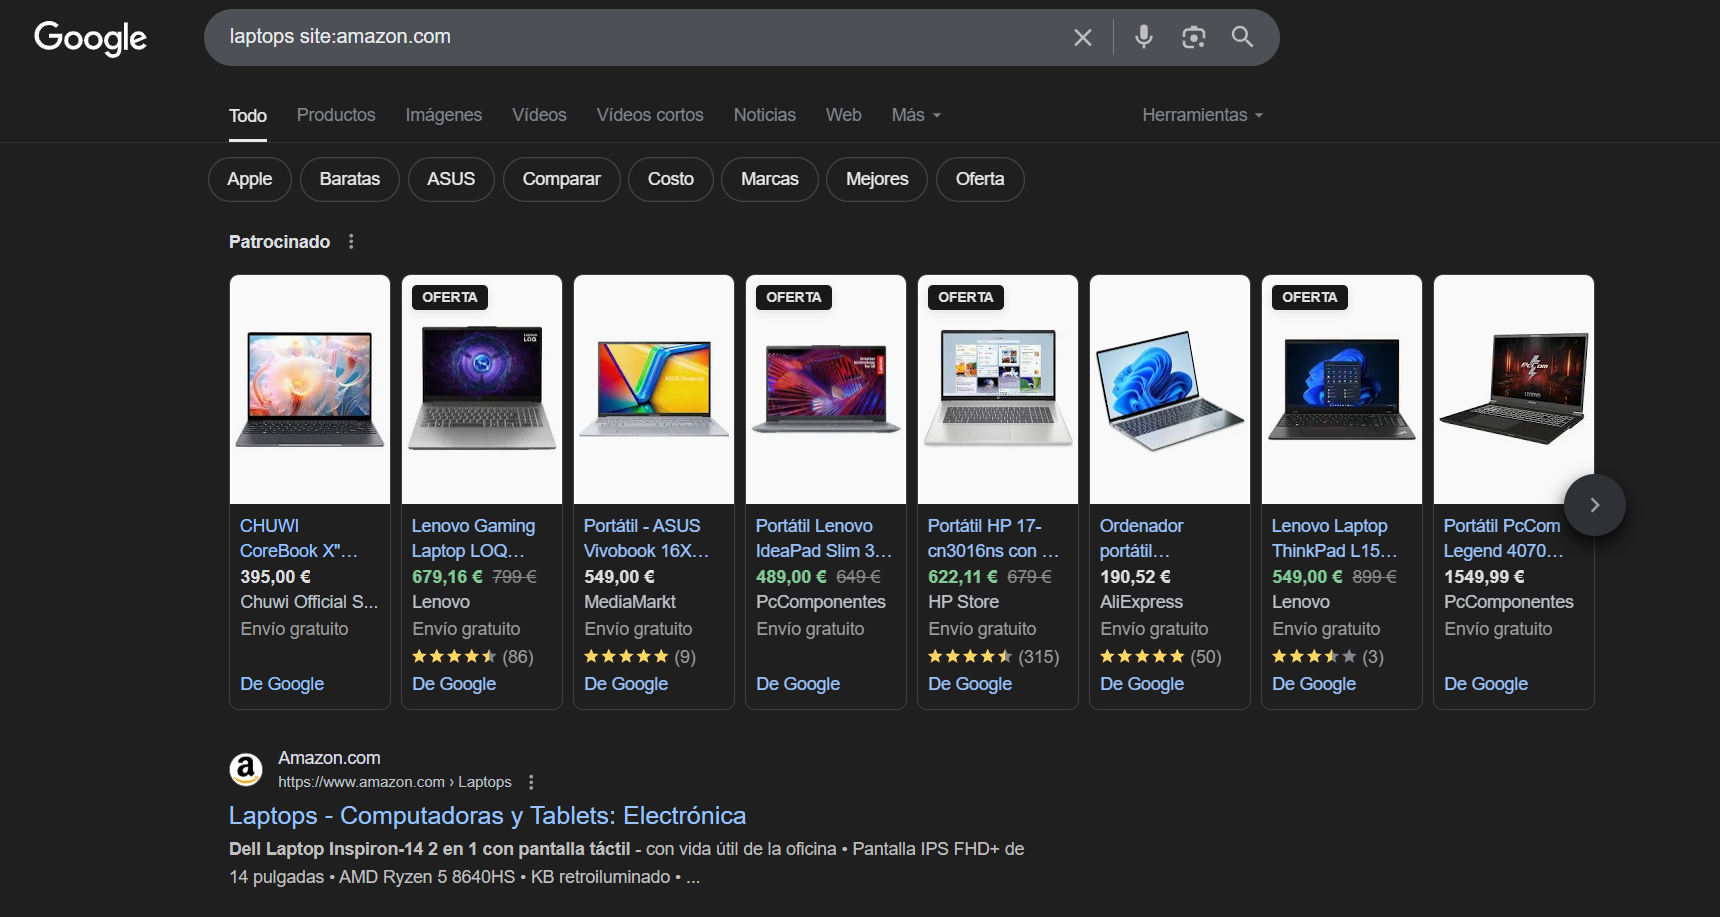
\includegraphics[scale=0.25]{figs/laptops.png}
    \caption{Búsqueda de portatil usando el query \emph{laptops site:amazon.com} en Microsoft Edge. 
    Los resultados de la búsqueda unicamente continen un producto perteneciente a Amazon, el resto
    son anuncios de otras páginas. Fuente: Elaboración propia.}
    \label{fig:laptops}
\end{figure}

Dados los retos que plantea este entorno, se han observado los siguientes
comportamientos:
\begin{itemize}
  \item \textbf{Descubrimiento del navegador}: Los agentes que poseen un flujo de razonamiento
  muy estático, como es el caso de \emph{Planex} y \emph{PlanexV2} e incluso \emph{RePlan},
  no son capaces de descubrir el navegador que deben utilizar, ya que se quedan atascados
  intentando abrir aplicaciones que no existen en el entorno, o bien
  intentando abrir aplicaciones que no son navegadores, como es el caso de \emph{browser.exe}.

  En el caso de \emph{RePlan}, el agente ha conseguido en una de las ejecuciones abrir
  el navegador, sin embargo en el resto del entorno no ha sido capaz de completar la tarea
  satisfactoriamente.

  \item \textbf{Interacción con el navegador}: El resto de agentes han sido capaces
  de descubrir el navegador instalado en el sistema, han conseguido realizar una
  busqueda en Edge, sin embargo han tenido problemas al no ser capaces de distinguir
  entre los resultados de la búsqueda y los anuncios de otras páginas.

  En el caso de \emph{Xplore}, el agente solo ha podido completar la tarea en una
  única ejecución, pues en el resto de ejecuciones ha gastado todo el tiempo de ejecución
  intentando recuperarse de paginas incorrectas.

  Por el contrario, en el caso de \emph{DarkVFR} el agente ha sido capaz de completar
  la tarea de forma eficiente sin equivocarse en los resultados de la búsqueda. Esto ha
  sido posible debido a que el agente a decidido aprovechar acciones alternativas a la 
  visión como las acciones basadas en OCR (Reconocimiento óptico de caracteres) para
  leer el contenido de la página y distinguir entre los resultados de búsqueda
  y los anuncios de otras páginas.

  \item \textbf{Añadir al carrito o comprar}: Todos los agentes que han alcanzado la página
  de Amazon han sido capaces de añadir el producto al carrito o comprarlo directamente. Esto
  se debe a que la mayoría de agentes han podido observar el botón de "Añadir al carrito" en 
  la página de búsqueda de portatiles de Amazon.

\end{itemize}


\begin{figure}[!h]
    \centering
    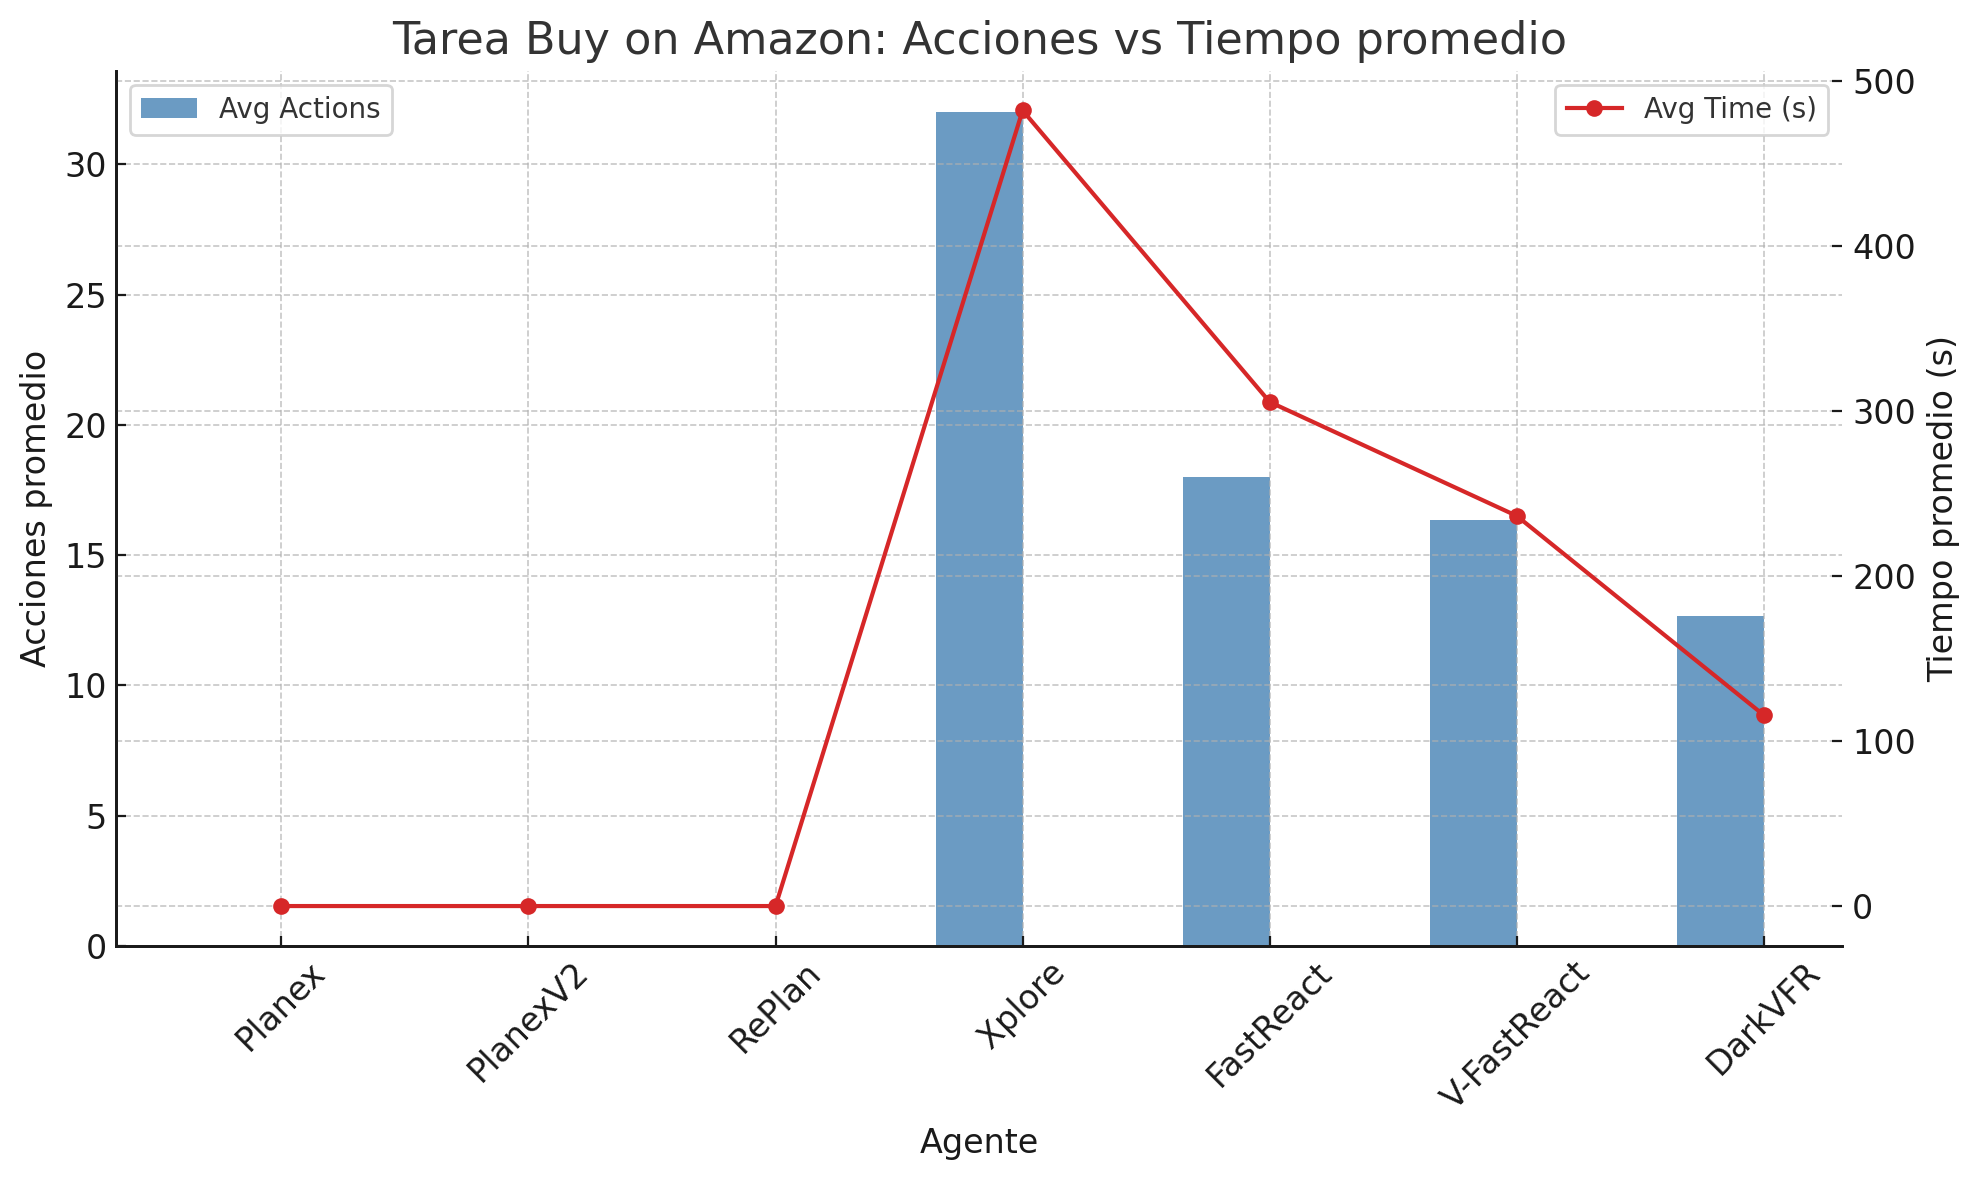
\includegraphics[scale=0.16]{figs/metrics-env-3.png}
    \caption{\small Rendimiento de los agentes (N. Acciones vs Tiempo promedio) en el 
    entorno \emph{Buy on Amazon}. Fuente: Elaboración propia.}
    \label{fig:env3}
\end{figure}

En la figura \ref{fig:env3} se puede observar como los agentes \emph{Planex}, \emph{PlanexV2}
y \emph{RePlan} no han sido capaces de completar la tarea, al no ser capaces de superar
los obstaculos de descubrimiento del navegador y de interacción con el mismo.

En el caso de \emph{Xplore}, el agente ha sido capaz de completar la tarea en una única
ejecución con un tiempo promedio de \emph{482 segundo (8 minutos)}, mientras que el resto 
de agentes ha sido capaces de resolver la tarea en menos de \emph{360 segundos (6 minutos)}.

En el caso de \emph{DarkVFR}, el agente obtiene un promedio record de 
\emph{115 segundos (1 minuto y 55 segundos)} con un número de acciones 
promedio de \emph{12 acciones}, lo que demuestra
la efectividad de las capacidades de visión y recuperación del agente para resolver
tareas complejas de forma eficiente y efectiva.

\subsection{Comparativa Global de Agentes}

Además del análisis detallado por entorno, resulta útil realizar una comparación
global para identificar tendencias generales de los agentes. Con este fin, 
la siguiente tabla presenta un resumen de las métricas de 
cada agente a lo largo de los tres entornos evaluados.

\begin{table}[!h]
\centering
\caption{Tiempo medio de resolución (s) por agente y entorno}
\label{tab:avg-times}
\begin{tabular}{p{3cm} c c c}
\toprule
\textbf{Agente} & \textbf{Hello World} & \textbf{Play a Song} & \textbf{Buy on Amazon} \\
\midrule
Planex           & 13.15     & --     & --     \\
PlanexV2         & 13.39     & --     & --     \\
RePlan           & 11.28     & 102.33 & --     \\
Xplore           & 14.19     & 31.33  & 482.11 \\
FastReact        & 10.68     & 64.63  & 305.46 \\
V-FastReact      & 9.58      & 23.81  & 236.41 \\
DarkVFR          & 5.71      & 15.82  & 115.68 \\
\bottomrule
\end{tabular}
\end{table}

En la Tabla~\ref{tab:avg-times} se presentan los tiempos medios de resolución,
en segundos, obtenidos por cada agente en los tres entornos evaluados:
\emph{Hello World}, \emph{Play a Song} y \emph{Buy on Amazon}. 

Como puede observarse, los agentes \textbf{Planex} y \textbf{PlanexV2} presentan
una ejecución eficiente en el entorno más sencillo (\emph{Hello World}), con
tiempos promedio de 13.15 y 13.39 segundos respectivamente. No obstante, ambos
agentes fallaron en resolver las tareas más complejas, lo que sugiere una falta
de adaptabilidad a entornos dinámicos que requieren razonamiento contextual o
verificación previa del estado del entorno.

Por el contrario, los agentes \textbf{Xplore} y aquellos basados en \textbf{FastReact} 
fueron capaces de completar satisfactoriamente los tres entornos, aunque con
diferencias relevantes en el tiempo de ejecución. \textbf{Xplore} muestra
tiempos considerablemente más altos, especialmente en el entorno \emph{Buy on
Amazon}, con un promedio de 482.11 segundos, lo cual indica una estrategia más
exhaustiva y posiblemente redundante. En comparación, \textbf{FastReact} logra
una mayor eficiencia con un tiempo medio de 305.46 segundos en ese mismo
entorno.

Finalmente, destaca el rendimiento de \textbf{DarkVFR}, que no solo completa
exitosamente todos los entornos, sino que además lo hace con los tiempos más
bajos en cada uno de ellos. En particular, alcanza un tiempo medio de apenas
115.68 segundos en la tarea más exigente, posicionándose como el agente más
eficiente del conjunto evaluado.

Estos resultados sugieren que, si bien la estrategia de ejecución directa puede
ser efectiva en entornos simples, la capacidad de verificación, adaptabilidad y
optimización en agentes como \textbf{DarkVFR} es determinante para un
rendimiento robusto en escenarios complejos.


\subsubsection{Consumo de tokens y coste estimado en “Buy on Amazon”}

\begin{table}[!h]
\centering
\caption{Tokens medios y coste medio estimado (€) por agente en “Buy on Amazon”}
\label{tab:tokens-cost-navigate-web}
\begin{tabular}{p{3cm} c c}
\toprule
\textbf{Agente}    & \textbf{Tokens promedio} & \textbf{Coste (€/ejecución)} \\
\midrule
Planex             & --       & --     \\
PlanexV2           & --       & --     \\
RePlan             & --       & --     \\
Xplore             & 512\,990 & 0.23   \\
FastReact          & 295\,400 & 0.13   \\
V-FastReact        & 223\,519 & 0.10   \\
DarkVFR            &  99\,649 & 0.04   \\
\bottomrule
\end{tabular}
\end{table}

La Tabla~\ref{tab:tokens-cost-navigate-web} presenta el consumo promedio de
tokens y el coste estimado por ejecución para cada agente durante la tarea
\emph{Buy on Amazon}. Dado que los experimentos se han llevado a cabo en un
entorno de bajos recursos (sistema empotrado), todas las llamadas a modelos 
de lenguaje se realizaron mediante APIs en la nube y por tanto, el coste
asociado se calcula en función del número de tokens consumidos.

El promedio de tokens mostrado corresponde al total consumido desde el envío del
primer prompt hasta la finalización exitosa de la tarea, incluyendo
razonamientos intermedios, reformulaciones y planificación. En todos los casos
se ha utilizado el modelo \texttt{gpt-4o-mini} de OpenAI, cuyo coste en el momento
de redacción de esta memoria es de \emph{0.45€ por millón de tokens}. Este modelo fue
seleccionado por ofrecer un equilibrio adecuado entre rendimiento y coste.

Tal como se aprecia en los datos, existe una relación directa entre el tiempo de
ejecución observado en la Tabla~\ref{tab:avg-times} y el número total de tokens
consumidos. Los agentes con estrategias más lentas y deliberativas tienden a
generar más interacciones con la LLM, lo que incrementa significativamente el
coste asociado. Esto es consistente con el diseño de los agentes: mientras que
la capa de ejecución y el espacio de acciones se ejecuta de forma prácticamente 
instantánea, la mayor parte del tiempo y consumo proviene del proceso de planificación y razonamiento
a través del modelo de lenguaje.

Entre todos los agentes evaluados, \textbf{DarkVFR} destaca no solo por ser el
más rápido, sino también por lograr la ejecución con el menor coste: tan solo
\emph{0.04€ por tarea}. Este rendimiento está alineado con su arquitectura, que
reutiliza razonamientos previos de forma optimizada y minimiza las llamadas
innecesarias a la LLM.

Como punto de referencia, se ha comparado este rendimiento con el de
\textsc{Operator}, un agente desarrollado por OpenAI. Si bien el número exacto
de tokens consumidos por \textsc{Operator} no es público, estimaciones
realizadas en condiciones locales utilizando el mismo modelo \texttt{gpt-4o-mini} 
indican un coste por tarea de navegación web que oscila entre \emph{0.30€} y \emph{0.50€}, es
decir, entre 7 y 12 veces más costoso que \textbf{DarkVFR}. Este resultado
refuerza la eficiencia del diseño propuesto en este trabajo, tanto desde una
perspectiva computacional como económica.

\subsubsection{Motivos de fallo}

\begin{table}[!h]
\centering
\caption{Motivos de fallo y número de ejecuciones fallidas (sobre 3)}
\label{tab:failure-reasons-count}
\begin{tabular}{p{2.5cm} p{3.5cm} p{3.5cm} p{3.5cm}}
\toprule
\textbf{Agente} & \textbf{Hello World} & \textbf{Play a Song} & \textbf{Buy on Amazon} \\
\midrule
Planex       & 0/3 (—)                  & 3/3 (out-of-actions) & 3/3 (out-of-time)    \\
PlanexV2     & 0/3 (—)                  & 3/3 (out-of-actions) & 3/3 (out-of-time)    \\
RePlan       & 0/3 (—)                  & 2/3 (out-of-actions) & 3/3 (out-of-actions) \\
Xplore       & 0/3 (—)                  & 0/3 (—)              & 2/3 (out-of-time)    \\
FastReact    & 0/3 (—)                  & 0/3 (—)              & 2/3 (out-of-time)    \\
V-FastReact  & 0/3 (—)                  & 0/3 (—)              & 0/3 (—)              \\
DarkVFR      & 0/3 (—)                  & 0/3 (—)              & 0/3 (—)              \\
\bottomrule
\end{tabular}
\end{table}

Finalmente, en la Tabla~\ref{tab:failure-reasons-count} se detallan los motivos
de fallo observados para cada agente en los diferentes entornos de prueba. En el
caso de \textbf{Planex}, \textbf{PlanexV2} y \textbf{RePlan}, los errores están
dominados por situaciones en las que el agente agotó el número máximo de
acciones permitidas (\emph{out-of-actions}). Esto sugiere una dificultad
estructural para explorar de forma eficiente el entorno o para identificar las
acciones relevantes necesarias para completar la tarea.

Por otro lado, los agentes \textbf{Xplore} y \textbf{FastReact} presentan fallos
principalmente asociados al agotamiento del tiempo disponible
(\emph{out-of-time}). Esto indica que, si bien son capaces de generar acciones
útiles e interactuar con el entorno de forma efectiva, sus estrategias de
exploración pueden resultar demasiado lentas o poco eficientes para completar
tareas complejas dentro del marco temporal impuesto.

En contraste, los agentes \textbf{V-FastReact} y \textbf{DarkVFR} han sido
capaces de completar satisfactoriamente los tres entornos sin registrar fallos.
En estos casos, las métricas de tiempo de ejecución y coste computacional se
convierten en los principales indicadores comparativos de rendimiento, ya que la
robustez funcional está garantizada.